% New supplementary material only. Does not alter or replace any existing section.
% Requires graphicx. Paths are relative to the Overleaf project root.
% Source statistics are copied without re-estimation from data/v4_confirmation_summary.json.
\section{A second Leduc cohort: allocation, stopping, and query-size ablations}
\label{add20260923:leduc:section}

\paragraph{Cohort identity and protocol.}
We evaluated a second, pre-registered cohort designed to make acquisition rules distinguishable after an earlier cohort produced identical EVSI, IVR, and LUCB decisions. This is an outcome-informed subsequent cohort, rather than an untouched first attempt. The eight-candidate family, query menu, budgets, and analysis were fixed before generating this cohort. Four pilot roots were included in 12 calibration roots, followed by 30 separate confirmation roots (15 equilibrator and 15 exploiter worlds; seeds 98000--98029). Opponent adaptation lengths were 1 and 8. The primary long-adaptation comparison used a cap of 16,384 HF hands. A paired query of size $n\in\{512,2048,4096\}$ costs $2n$ hands; fixed-size comparators use $n=4096$. Selection methods were replayed on the same sealed banks, and deployment regret was scored against exact OpenSpiel expected returns, including the incumbent as a no-update option. PIVOT-KG denotes the joint-Gaussian knowledge-gradient implementation used in this cohort; these numbers are not results for a separately implemented author baseline.

\paragraph{Mechanism and allocation.}
The mean root-level reversal rate among proxy-positive candidates increased from 2.50\% under short adaptation to 51.67\% under long adaptation (Figure~\ref{add20260923:leduc:reversal}). At the primary budget, PIVOT-KG menu reduced mean selection regret from 0.043153 for expected Uniform fixed to 0.013264 (Table~\ref{add20260923:leduc:methods}). The pre-specified primary paired selected-gain difference was $+0.029889$, with saved 95\% root-bootstrap interval $[0.005868,0.058099]$ and sign-flip $p=0.02148$. Expected Uniform averages exactly over all equally likely fixed-size query subsets. The comparison against the separately registered single Uniform draw had interval $[-0.010829,0.067025]$ and did not establish an advantage. Method-level intervals in Figure~\ref{add20260923:leduc:regret} do not substitute for these paired contrasts.

\paragraph{Stopping and the HF menu.}
Early stopping reduced mean HF consumption from 16,384 to 12,083.2 hands, a saving of 4,300.8 hands (26.25\%; Figure~\ref{add20260923:leduc:stopping}). The saved paired hands-difference interval is $[-6007.4667,-2662.4]$. Observed selected-gain differences were zero in all 30 confirmation roots. This is a query-sample saving in offline replay, not a measured reduction in total bank-generation cost, runtime, or cloud charges, and it is not a guarantee of losslessness on other tasks. The query-size menu did not improve selected gain over fixed-size PIVOT-KG: the menu-minus-fixed difference was $-0.013161$ with interval $[-0.029576,0]$. The protocol's menu version remains the primary method; the stronger fixed-size point estimate does not replace it retrospectively.

\paragraph{Other component findings.}
Table~\ref{add20260923:leduc:contrasts} and Figure~\ref{add20260923:leduc:components} retain the null and negative component comparisons. The results do not establish that the menu selector outperforms IVR or LUCB, or that paired queries improve final selected gain over the unpaired variant. Exact versus noisy calibration produced equal selected gains for the observed roots; the noisy-calibration allocation contrast against expected Uniform was positive. Secondary intervals are pointwise and have no multiplicity adjustment. LORO gates C1--C3 passed, with held-out 95\% predictive coverage 0.9583 and 0.9688 for short and long adaptation. The confirmation summary's gate fields are null; the gate evidence comes from the separately archived LORO summary. All statistics below are the previously saved results; this supplement performs no new statistical estimation.

\begin{table}[t]
\centering
\caption{All 13 reported methods at long adaptation and the primary cap, with exact calibration and 30 confirmation roots. Lower regret and higher selected deployment gain are better. All-HF is a four-times-budget reference, while no-HF and proxy-only use zero new HF hands. Uniform fixed is an exact query-subset expectation; Uniform small uses the saved 64-draw Monte Carlo average.}
\label{add20260923:leduc:methods}
\small
\begin{tabular}{lrrr}
\hline
Method & Mean regret & Mean gain & Mean HF hands \\
\hline
PIVOT-KG fixed & 0.000104 & 0.119670 & 16,384 \\
Top-proxy fixed & 0.004017 & 0.115757 & 16,384 \\
All-HF fixed (reference) & 0.007277 & 0.112496 & 65,536 \\
PIVOT-KG menu & 0.013264 & 0.106509 & 16,384 \\
PIVOT-KG menu + stopping & 0.013264 & 0.106509 & 12,083.2 \\
LUCB fixed & 0.018902 & 0.100871 & 16,384 \\
IVR menu & 0.021306 & 0.098467 & 16,384 \\
IVR fixed & 0.021384 & 0.098389 & 16,384 \\
Uniform small & 0.023825 & 0.095948 & 16,384 \\
PIVOT-KG menu, unpaired & 0.026767 & 0.093006 & 16,384 \\
Uniform fixed (expectation) & 0.043153 & 0.076621 & 16,384 \\
Calibrated, no HF & 0.258765 & $-0.138991$ & 0 \\
Proxy-only & 0.670558 & $-0.550785$ & 0 \\
\hline
\end{tabular}
\end{table}


\begin{table}[t]
\centering
\caption{Saved paired component contrasts at the primary cap, $N=30$. All rows report selected-gain differences except the explicitly labeled HF-hands row. Positive values favor the first term. $H_A$ versus expected Uniform is the pre-specified primary comparison. Remaining intervals are unadjusted; zero-width intervals describe these observed roots only.}
\label{add20260923:leduc:contrasts}
\small
\resizebox{\linewidth}{!}{%
\begin{tabular}{llrr}
\hline
ID & Contrast & Mean difference & 95\% interval \\
\hline
$H_A$ & Menu $-$ expected Uniform & $+0.029889$ & $[0.005868,0.058099]$ \\
$H_A$ & Menu $-$ registered Uniform draw & $+0.022629$ & $[-0.010829,0.067025]$ \\
$H_B$ & Menu $-$ IVR menu & $+0.008042$ & $[0,0.021976]$ \\
$H_{B2}$ & Menu $-$ LUCB fixed & $+0.005638$ & $[-0.024932,0.049394]$ \\
$H_{B3}$ & Menu $-$ top-proxy fixed & $-0.009248$ & $[-0.026208,0.002945]$ \\
$H_C$ & Paired $-$ unpaired menu & $+0.013503$ & $[-0.001915,0.032026]$ \\
$H_D$ & Exact $-$ noisy calibration & $0$ & $[0,0]$ \\
$H_D$ & Noisy menu $-$ expected Uniform & $+0.028791$ & $[0.006160,0.054610]$ \\
$H_E$ & Stopping $-$ full menu (gain) & $0$ & $[0,0]$ \\
$H_E$ & Stopping $-$ full menu (HF hands) & $-4300.8$ & $[-6007.4667,-2662.4]$ \\
$H_F$ & Menu $-$ fixed size & $-0.013161$ & $[-0.029576,0]$ \\
$H_G$ & Long $-$ short allocation contrast & $+0.029889$ & $[0.005868,0.058099]$ \\
\hline
\end{tabular}%
}
\end{table}


\begin{figure}[t]
\centering
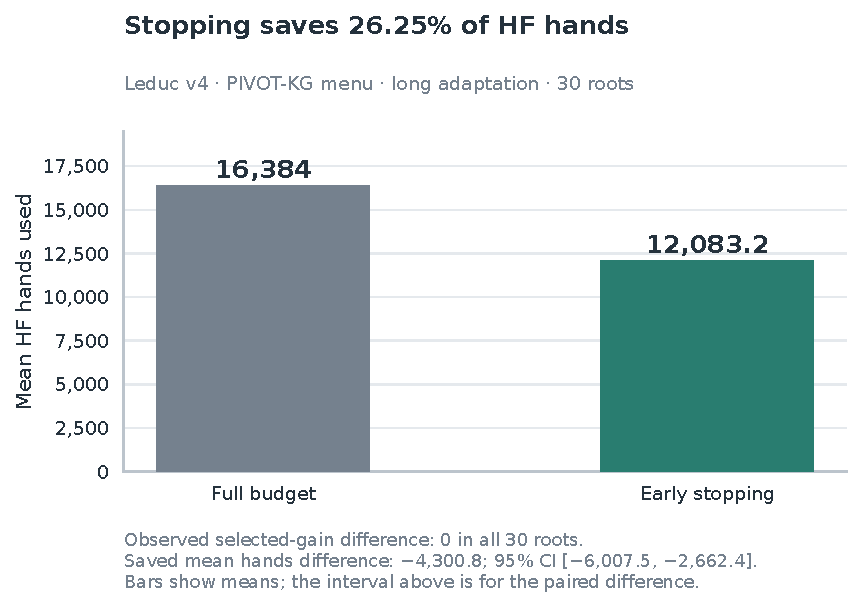
\includegraphics[width=0.84\linewidth]{additions_20260923/leduc/figures/03_stopping_budget.pdf}
\caption{HF hands consumed by PIVOT-KG menu with and without stopping. Means are shown without invented per-bar intervals; the saved paired difference interval is stated separately. Final selected-gain differences were zero for all 30 observed roots. This measures query-sample use on sealed banks, not end-to-end computational cost.}
\label{add20260923:leduc:stopping}
\end{figure}

\begin{figure}[t]
\centering
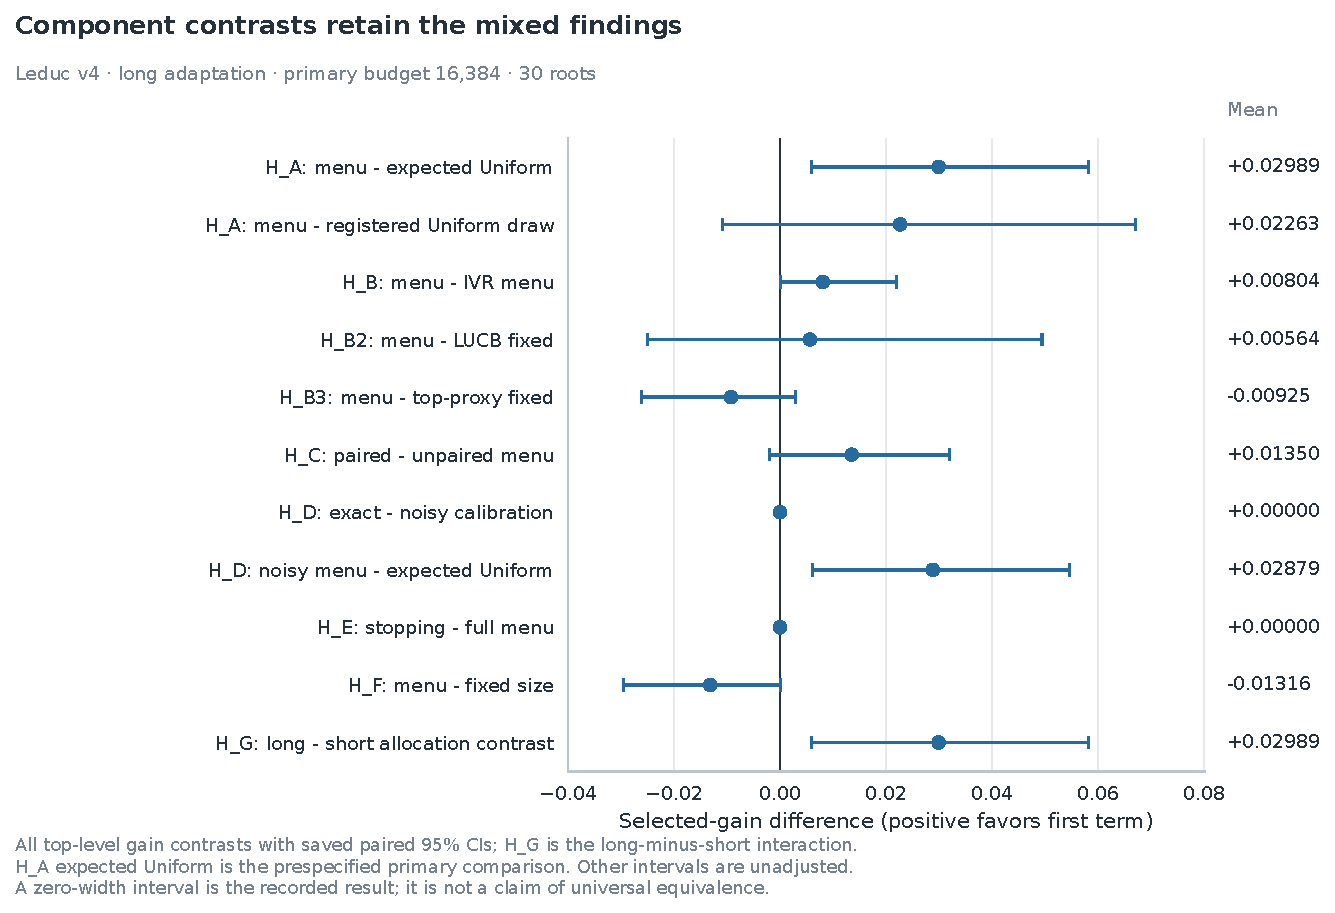
\includegraphics[width=\linewidth]{additions_20260923/leduc/figures/05_v4_component_contrasts.pdf}
\caption{All saved top-level gain contrasts, including the menu-versus-fixed null/negative finding. Error bars are saved paired root-bootstrap 95\% intervals; secondary comparisons are unadjusted. The HF-hands contrast is reported separately.}
\label{add20260923:leduc:components}
\end{figure}

\begin{figure}[t]
\centering
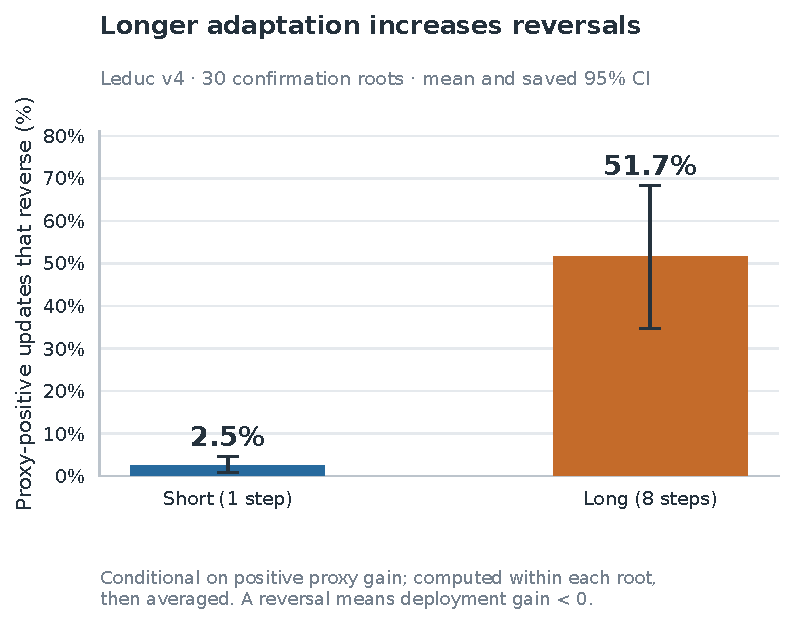
\includegraphics[width=0.84\linewidth]{additions_20260923/leduc/figures/01_proxy_deployment_reversal.pdf}
\caption{Proxy-positive improvement reversal in the second Leduc cohort. Within each root, the rate is the fraction of candidates with positive proxy gain whose deployment gain is negative. Bars show the mean of 30 root-level rates and the saved 95\% root-bootstrap intervals for 1-step and 8-step adaptation. Candidates within a root are not independent experimental units.}
\label{add20260923:leduc:reversal}
\end{figure}

\begin{figure}[t]
\centering
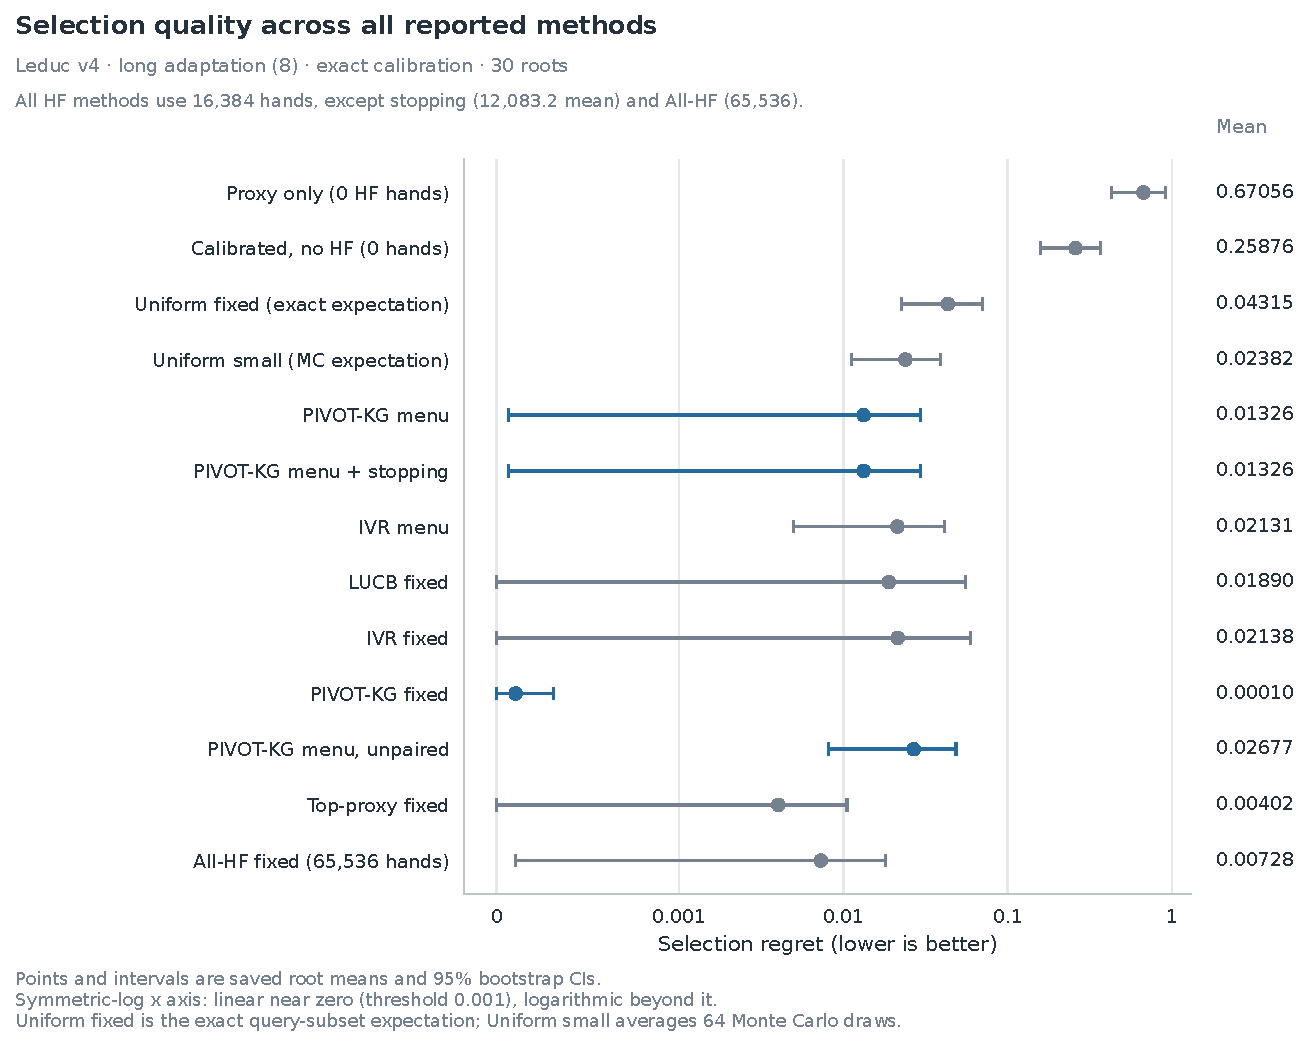
\includegraphics[width=\linewidth]{additions_20260923/leduc/figures/02_selection_regret_all_methods.pdf}
\caption{All 13 reported methods and saved 95\% root-bootstrap intervals at long adaptation. Regret is the best attainable deployment gain, including retaining the incumbent, minus the selected gain. Budget exceptions are labeled. The symmetric-log axis is linear within 0.001 of zero; visual distances are not on a globally linear scale. Paired method comparisons are reported in Table~\ref{add20260923:leduc:contrasts}.}
\label{add20260923:leduc:regret}
\end{figure}

\subsection{E1: all seven pre-specified settings}
\label{add20260923:leduc:e1-section}
The separate E1 suite used the earlier candidate family and its own protocol-defined Uniform comparator, with 30 confirmation roots per setting and a primary budget of 16,384 HF hands. It must not be pooled with the v4 cohort or interpreted as the same expected-Uniform experiment. Figure~\ref{add20260923:leduc:e1-all} retains all seven settings and both the frozen and corrected analyses of the same saved worlds. These two analyses are not independent replications. Table~\ref{add20260923:leduc:e1-table} reports the corrected contrasts. Pointwise lower bounds are positive for four settings; the $\eta=0.05$ point estimate is negative, the $\eta=0.40$ interval touches zero, and the $P(\mathrm{exploiter})=0.95$ effect is zero. These secondary intervals are not adjusted for the seven settings; they do not establish a joint family-wide significance claim or a monotonic relation between response strength and PIVOT value.

\begin{table}[t]
\centering
\caption{All seven E1 corrected PIVOT-KG-minus-Uniform selected-gain contrasts. Saved pointwise 95\% root-bootstrap intervals, 30 roots per setting. These results are separate from the second-cohort v4 main comparison.}
\label{add20260923:leduc:e1-table}
\small
\begin{tabular}{lrr}
\hline
Setting & Mean gain difference & 95\% interval \\
\hline
$\eta=0.05$ & $-0.014819$ & $[-0.032008,0.000248]$ \\
$\eta=0.10$ & $+0.033218$ & $[0.006116,0.066191]$ \\
$\eta=0.25$ & $+0.014826$ & $[0.002280,0.031415]$ \\
$\eta=0.40$ & $+0.001501$ & $[0,0.004504]$ \\
$P(\mathrm{exploiter})=0.80$ & $+0.023550$ & $[0.003317,0.052706]$ \\
$P(\mathrm{exploiter})=0.95$ & $0$ & $[0,0]$ \\
Continuous mixture & $+0.051202$ & $[0.003287,0.112217]$ \\
\hline
\end{tabular}
\end{table}


\begin{figure}[t]
\centering
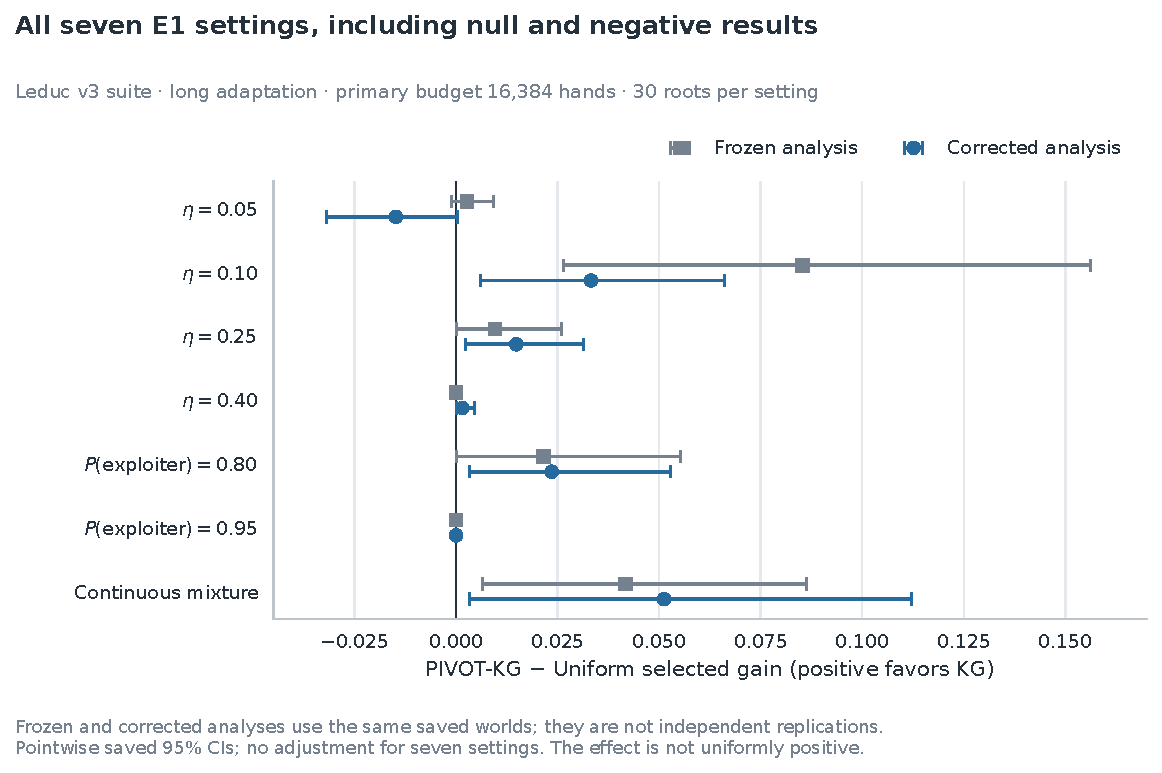
\includegraphics[width=\linewidth]{additions_20260923/leduc/figures/04_e1_all_seven_settings.pdf}
\caption{All seven E1 settings, including null and negative results. Frozen and corrected analyses use the same saved worlds and differ in the calibration-noise treatment; they are not independent replications. Error bars are the saved pointwise 95\% root-bootstrap intervals without multiplicity adjustment. The primary budget is 16,384 HF hands in each setting.}
\label{add20260923:leduc:e1-all}
\end{figure}
